\section{Introduction}
\label{sec:introduction}

% state the learning objective 
The objective of this laboratory assignment was to simulate and create an acdc converter
that would minimize the cost of the components while decreasing the ripple of output.
We used Octave for a theoretical analysis of the circuit and Ngspice to simulate it.
The values of both analysis are compared at the end of this document.
The units of the cost is MU (monetary unit).
The merit of our circuit is given by the following expression:

\begin{equation}
    M = \frac{1}{cost(ripple(v_0)+average(v_0-12)+10^{-6})}
\end{equation}\par

Where: \par
cost = cost of Resistors + cost of Capacitors + cost of Diodes \par
cost of Resistor = 1 MU per kOhm \par
cost of Capacitor = 1 MU per $\mu$ F \par
cost of Diodes = 0.1 MU per diode \par

\vspace{10mm}
The circuit we built is presented in figure \ref{fig:circuit}.
The transformer in the left side is considerer to be ideal and the ration N1/N2 is approximated to 17.577.
This means that we considered an AC source of 13.0855 V (50Hz) for the rest of the circuit in the right side.

\vspace{-4mm}
\begin{figure}[ht] \centering
    \caption{ACDC converter circuit}
    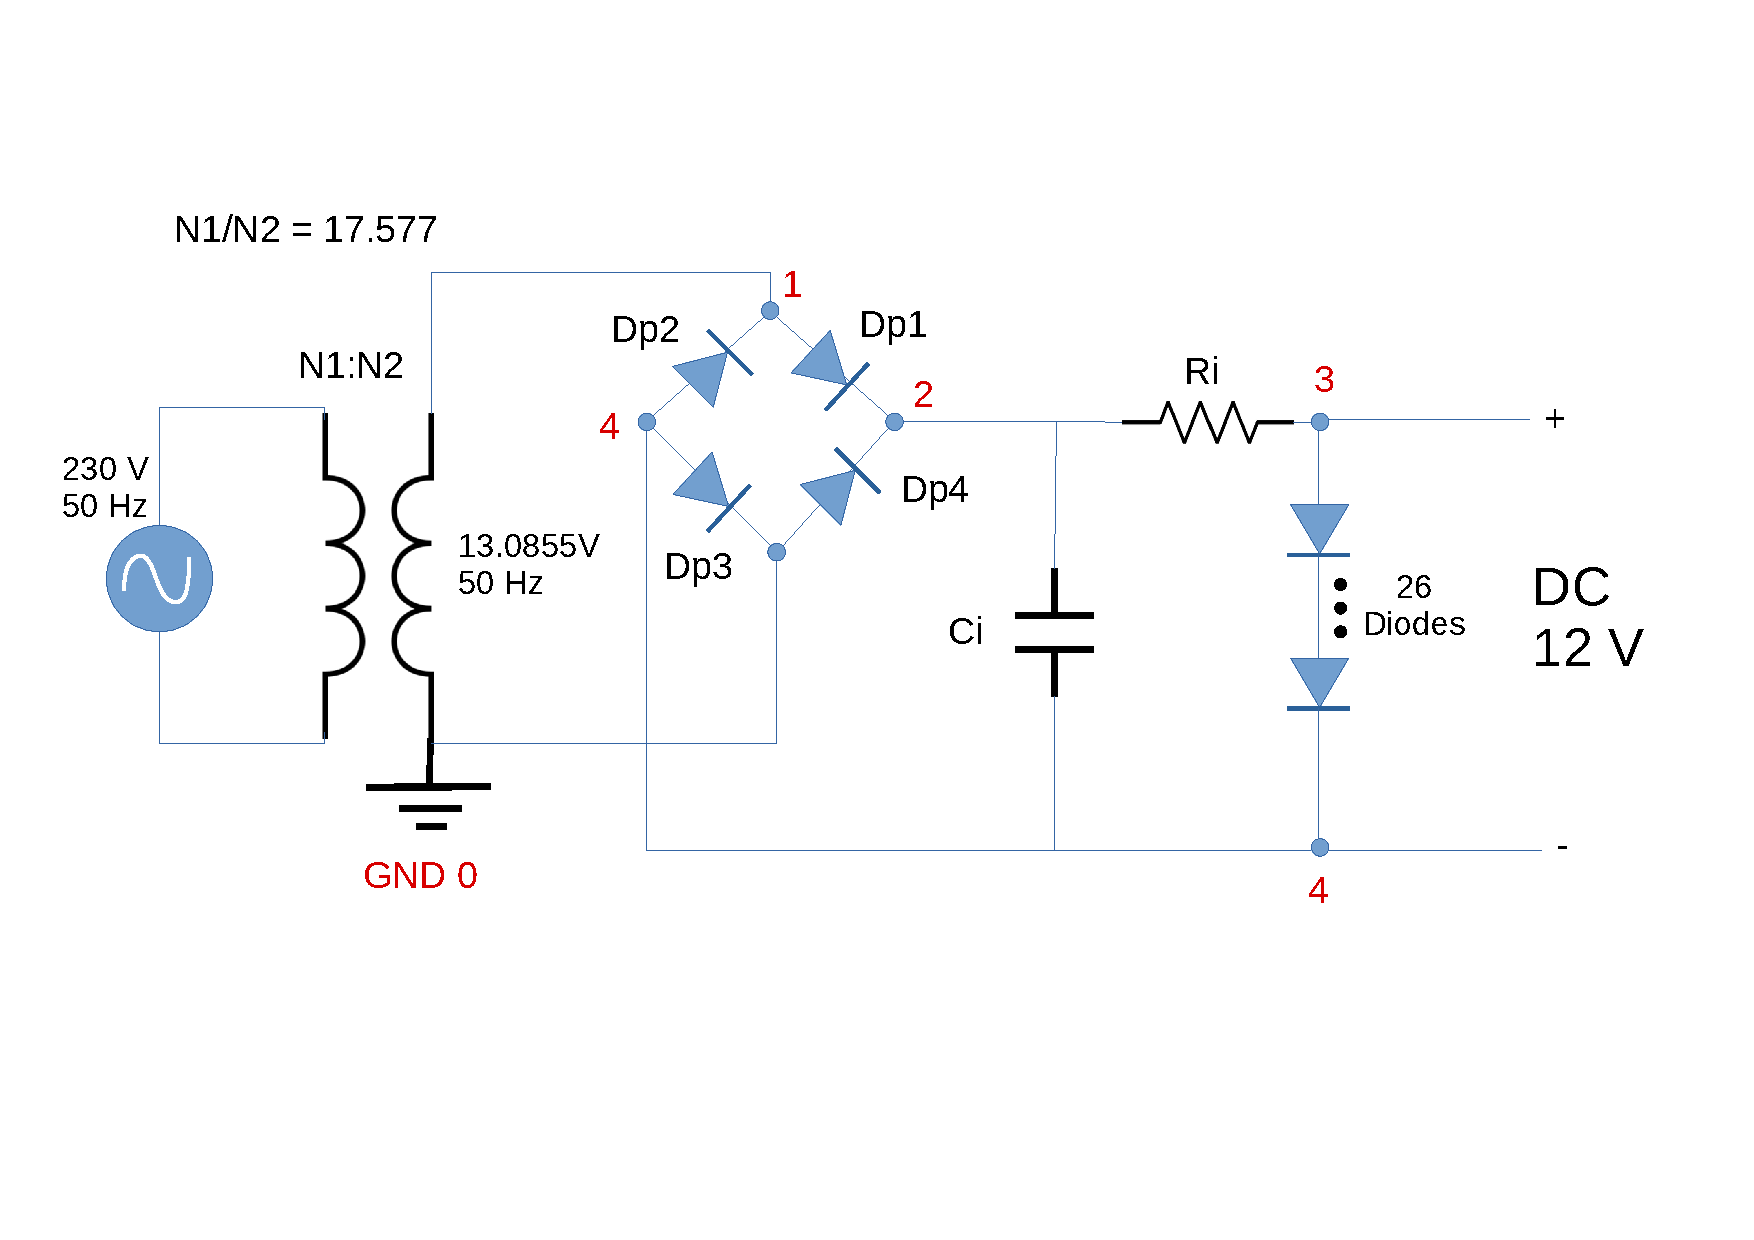
\includegraphics[width=0.8\linewidth]{circuit.pdf}
    \label{fig:circuit}
\end{figure}

\vspace{-6mm}
Components used and respective price are presented in table \ref{tab:material}:
\vspace{5mm}
\begin{table}[ht]
    \centering
    \begin{tabular}{|c|c|c|}
      \hline    
      {\bf Component} & {\bf Quantity or Value} & {\bf Cost} \\ \hline
      Resistor (Ri) & 13.6 kOhm & 13.6 MU \\ \hline
      Capacitor (Ci) & 8 uF & 8.0 MU \\ \hline
      Diodes (Dp1-Dp30) & 30 & 3.0 MU \\ \hline
      Total & - & 24.6 MU \\ \hline
    \end{tabular}
    \vspace{5mm}
    \caption{Electrical Components used and respective cost in MU}
    \label{tab:material}
  \end{table}